\chapter{Limbajul Java și optimizarea acestuia}

În acest capitol vom descrie cum putem adapta optimizarea eliminării de metode pentru limbajul Java.
Scopul final este să implementăm algoritmul descris la sfârșitul capitolului `Optimizări de dimensiune'~\ref{capitolul_optimizari_de_dimensiune}.

\section{Optimizarea limbajului Java}

% În aceasta parte vom urmări implementarea algoritmului descris la sfârșitul
% capitolului `Optimizări de dimensiune'~\ref{capitolul_optimizari_de_dimensiune}.

\subsection{Preliminarii}

Java este un limbaj dinamic. Acest lucru înseamnă posibilitatea de a modifica
codul în timpul rulării, sau de a apela cod în mod dinamic la rulare: aceasta
este partea de `reflecție' a limbajului Java.

Utilizarea acestor caracteristici face abordarea noastră de analiză
statică imposibilă, întrucât optimizatorul ar putea elimina metode care nu sunt
apelate în mod explicit în cod, însă care ajung să fie referențiale în mod
dinamic la rulare.

Prin urmare, în continuarea lucrării vom presupune că toate proiectele Java cu
care lucrăm nu se folosesc de niciun mod de a schimba structura codului în
timpul rulării. În caz contrar, optimizatorul nu mai oferă nicio garanție asupra
corectitudinii optimizărilor realizate.

Restul lucrării va presupune că această condiție este respectată.


\subsection{Determinarea punctului de intrare}

Un proiect Java este format dintr-o mulțime de clase.
Punctul \texttt{main} al proiectului este reprezentat de funcția
denumită \texttt{main} \cite{java_main}, cu antetul

\begin{lstlisting}[language=Java]
public static void main(String [] args)
\end{lstlisting}

Într-un proiect trebuie să existe o singură astfel de metodă, care să aparțină
unei clase a proiectului.

Pentru a găsi metoda \texttt{main}, sunt scanate toate fișierele
clasa care fac parte din proiect, și sunt analizate listele de
metode ale acestora.

Acesta este pseudocodul pentru această operație:
\begin{lstlisting}[language=Python, label=main_method]
def main_method(p: Proiect):
    ret = None
    for classfile in p.classfiles:
        if "main" in p.methods():
            if ret:
                assert False, "Am gasit mai multe metode main!".
            ret = p.method_of_name("main")
    if not ret:
        assert False, "Proiectul trebuie sa aiba o metoda main!".
    return ret
\end{lstlisting}

\subsection{Găsirea apelurilor de funcții}

Pentru a determina ce funcții sunt apelate din cadrul unei metode \texttt{m},
vom inspecta atributul de cod al lui \texttt{m}.
Dintre instrucțiunile conținute vom fi interesați doar de cele ce implică
apeluri de funcții - familia invoke*.

Odată găsite instrucțiunile de invocare de funcții, este necesar să rezolvăm
referințele conținute de acestea, întrucât în reprezentarea interna a JVM-ului,
o metodă este referențială pur simbolic, prin șiruri de caractere.

\subsection{Rezolvarea metodelor speciale}

Acest tip de rezolvare a metodelor este necesar atunci când întâmpinam
instrucțiunea \textbf{invokespecial}.

Prin metode speciale înțelegem funcții precum constructorul unei clase sau
funcții private.

Pentru scopul acestei lucrări, nu vom elimina constructorii,
întrucât asta ar înseamna eliminarea unei clase cu totul (i.e.,
singurul caz în care putem elimina constructorul unei clase este
când clasa nu este instanțiată niciodată).

Metodele private, în schimb, vor fi tratate ca niște funcții normale.

\subsection{Rezolvarea metodelor dinamice}

Din versiunea 7 a limbajului Java a fost introdusă instrucțiunea
\textbf{invokedynamic}.
Aceasta instrucțiune este folosită în rezolvarea referințelor de metode la
rulare - similar cu conceptul de "duck typing" din limbajele dinamice.
Deoarece am făcut presupunerea că proiectele cu care lucrăm nu vor utiliza
reflecția sau invocarea dinamică a codului, această instrucțiune nu va
fi întâlnită.

\subsection{Rezolvarea metodelor statice}

Metodele statice sunt cele mai simple de rezolvat: referința către o astfel de
metodă indică numele metodei, tipul metodei, cât și clasa din care face parte și
de unde este invocată.
Aceste metode sunt rezolvate direct la compilare, deci tuplul (nume, tip, clasă)
identifică în mod unic o metodă statică.

\subsection{Rezolvarea metodelor virtuale}

În Java, toate metodele de instanță (non-statice) sunt polimorfice la rulare
(Eng. Run time polymorphism).
Cu alte cuvinte, la compilare se știu numele, tipul metodei și clasa unde
metoda este definită, însă \textbf{nu} și clasa de unde este invocată.

Aceasta este cea mai comună operație, și corespunde instrucțiunii
\textbf{invokevirtual}.

De exemplu, pentru programul
\begin{lstlisting}[language=Java, numbers=left, label=program_metode_virtuale]
public class Main {
    static private class One extends Other {
        public void foo() {
            System.out.println("foo() of One");
        }
    }

    public static void bar(Other o) {
        o.foo();
    }

    public static void main(String[] args) {
        Other o = new One();
        bar(o);
    }
}

public class Other {
    public void foo() {
        System.out.println("foo() of Other");
    }
}
\end{lstlisting}
format din concatenarea fișierelor din testul \texttt{fixtures/project4},
apelul de pe linia 9 către metoda foo este un apel polimorfic.

În codul de JVM, instrucțiunea corespunzătoare este:

\texttt{invokevirtual \#2                  // Method Other.foo:()V}

Unde poziția 2 din tabela de constante este o referință către o metodă cu numele
de \texttt{foo} cu tipul \texttt{void foo()}, definită în clasa \texttt{Other}.

\texttt{\#2 = Methodref          \#22.\#23        // Other.foo:()V}

Deși metoda \texttt{foo} este definită inițial în clasa \texttt{Other}, la
rulare va fi apelată versiunea definită în subclasa \texttt{One}.

În implementarea JVM-ului, în vârful stivei mașinii se va afla o referință către instanța obiectului
a cărui metodă este apelată. În cazul programului nostru, pe stivă se va afla o
referință către variabila \texttt{o}, de tipul \texttt{Other}, definită pe linia
13 a programului.

Pentru rezolvarea metodei virtuale, JVM-ul se asigură că tipul lui \texttt{o},
adică \texttt{Other}, este un moștenitor al clasei de care aparține metoda
\texttt{One}. În caz că tipul \texttt{Other} definește chiar el metoda
căutată, mașina va folosi definiția respectivă.
În caz contrar, mașina virtuală va cauta recursiv metoda în super clasa lui
\texttt{Other}. În cazul în care căutarea recursivă a ajuns până la o clasa fără
super (singura astfel de clasa este \texttt{Object}), mașina virtuală va emite o
eroare.

\subsection{Rezolvarea metodelor de interfața}

Ultimul tip de invocare a metodelor corespunde instrucțiunii
\textbf{invokeinterface}, și corespunde apelării unei funcții declarate în cadrul
unei interfețe.

De exemplu, pentru programul
\begin{lstlisting}[language=Java, numbers=left]
public interface I {
    public void foo();
}
public class Main {
    static private class C implements I{
        public void foo() {
            System.out.println("foo() of C");
        }
    }

    public static void bar(I i) {
        i.foo();
    }

    public static void main(String[] args) {
        I i = new C();
        bar(i);
    }
}
\end{lstlisting}
format din fișierele testului \texttt{fixtures/project5},
apelul de pe linia 11 către metoda foo este un apel polimorfic pe interfețe.

În codul de JVM, instrucțiunea corespunzătoare este:

\texttt{invokeinterface \#2,  1            // InterfaceMethod I.foo:()V}

Unde slotul 2 din tabela de constante este o referința către o metoda de
interfața cu numele de \texttt{foo} cu tipul \texttt{void foo()}, definită în
interfața \texttt{I}.
\texttt{\#2 = InterfaceMethodref \#22.\#23        // I.foo:()V}

Deși metoda \texttt{foo} este declarată inițial în interfața \texttt{I}, la
rulare va fi apelată versiunea definită în subclasa \texttt{C}.

Pentru rezolvarea referințelor către metode de interfață, se va aplica un algoritm similar cu
cel de la rezolvarea referințelor de metode virtuale: căutare recursivă în
lanțul de moșteniri al clasei asupra căruia se execută metoda.

\subsection{Algoritmul de rezolvare al referințelor metodelor}

Putem defini în pseudo cod algoritmul de rezolvare al referințelor către metode
virtuale și către metode de interfața astfel:

\begin{lstlisting}[language=Python, label=from_symbolic_reference]
def from_symbolic_reference(
    class, method_name, method_type) -> Method:
    if class is Object:
        return None
    for m in class.methods():
        if m.name == method_name and m.type == method_type:
            return m
# Nu am putut sa rezolvam referinta in clasa curenta,
# incercam in super.
    return resolve_reference(
        class.super_class, method_name, method_type)
\end{lstlisting}

Metoda exactă care este executată de o astfel de instrucțiune nu poate fi știută
decât abia la timpul rulării (e.g., pentru programul~\ref{program_metode_virtuale}
nu putem știi în timpul analizei statice dacă va fi apelată metoda
\texttt{Other::foo()} sau metoda \texttt{One::foo()}).

\subsection{Superșirul de execuție și polimorfismul de execuție}

Vom reconsidera superșirul de execuție definit la \ref{supersirul_de_executie}
și graful apelurilor, definit la \ref{graful_apelurilor}.

La momentul analizei statice nu știm tipul exact al unei referințe.
O referință către o interfață poate să conțină orice obiect care implementează
acea interfață, sau o referință către o clasă \s{C} poate conține fix clasa
\s{C}, sau orice clasă care o are pe \s{C} ca strămoș.
, care determină ce funcții
Prin urmare, vom extinde superșirul de execuție ca să reflecte aceste
posibilități.
Mai precis, pentru fiecare apel de funcții polimorfice (virtuale prin
\textbf{invokevirtual} sau de interfață prin \textbf{invokeinterface}), vom
considera toate metodele posibile care pot fi referențiate.

De exemplu, pentru programul~\ref{program_metode_virtuale}, vom considera toate
posibilitățile de rezolvare ale apelului către foo(), atât \texttt{Other::foo()},
cat și \texttt{One::foo()}.

\subsection{Graful de apeluri și polimorfismul de execuție}

Acum că am adaptat superșirul de execuție pentru polimorfismul de execuție, este
nevoie să extindem și graful de apeluri.

Pentru acest lucru, în cadrul unei rezoluții vom considera nu numai metoda
direct referențială, ci toate metodele pe care superșirul de execuție le-ar
putea rezolva ca posibili candidați.

Vom spune ca metoda m este un candidat pentru rezoluția metodei q dacă în
rezolvarea unei referințe către q, superșirul de execuție va considera și metoda
m.

Proprietatea de a fi candidat este o relație reflexivă și tranzitivă, însa nu și
simetrică.

Această relație este echivalentă cu: metoda m este un candidat pentru rezoluția
metodei q dacă:
\begin{enumerate}
    \item q este o metodă a unei interfețe, iar m implementează direct sau
        tranzitiv interfața respectivă.
    \item q este o metodă a unei clase, iar m moștenește direct sau tranzitiv
        clasa respectivă.
\end{enumerate}

În continuare, vom nota cu $cand(m)$ \label{cand} tot candidații lui m. Din faptul ca este o
relație reflexiva, m aparține mulțimii $cand(m)$.

Graful de apeluri trebuie schimbat astfel încât să includă și candidații unei
metode: în loc să tragem o singură muchie de la metoda p care face invocarea, la
metoda m care este invocată, vom trage mai multe muchii: de la p la toate
metodele candidate pentru m --- $cand(m)$.

\subsection{Noul algoritm pentru eliminarea funcțiilor}

În această parte, vom adapta algoritmul de eliminare a funcțiilor, definit
anterior la \ref{algoritm_naiv_pentru_eliminare}.
În particular, vom actualiza modul de calculare al funcțiilor accesibile:

\begin{lstlisting}[language=Python, label=reachable_methods_in_java]
def reachable_methods_in_java(main: Method) -> [Method]:
    coada = [main]
    at = 0
    while at < size(coada):
        m = coada[at]
        at = at + 1
        for next in direct_calees(m):
            for c in cand(next):
                if c not in coada:
                    coada.push(c)
    return coada
\end{lstlisting}


Iar procedura de optimizare va rămâne identică:

\begin{lstlisting}[language=Python, label=optimize_for_size_in_java]
def optimize_for_size_in_java(p: Program) -> Program:
    main = p.main_method()
    used_methods = reachable_methods(main)
    for m in p.all_methods():
        if m not in used_methods:
            p.remove_method(m)
    return p
\end{lstlisting}

\section{Implementarea în C++}

În această secțiune, voi face legătura între algoritmii în pseudocod descriși
anterior și implementarea în C++.
Codul sursă este disponibil pe GitHub~\cite{project_sourcecode} este documentat,
cu comentarii, iar programul Doxygen poate fi folosit pentru a genera
documentație pentru proiect.
În continuare, voi descrie legătura dintre implementarea în C++, și
algoritmii în pseudocod descriși anterior.

Partea relevantă a proiectului pentru problema optimizării este conținută în
două clase: Method și Project.

\begin{figure}[H]
	\centering
	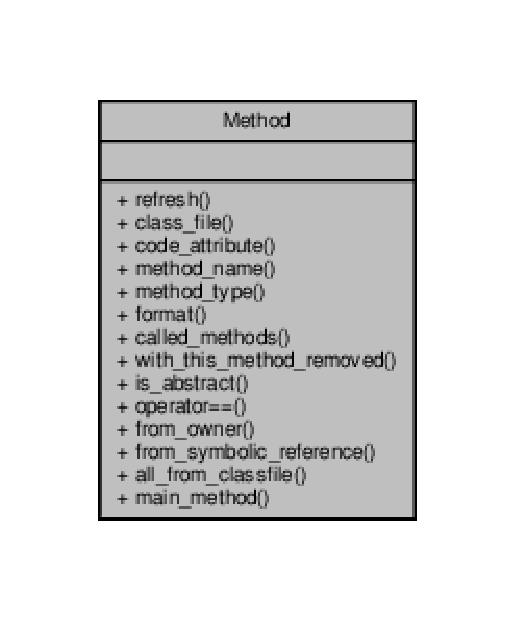
\includegraphics[width=0.5\textwidth]{classMethod__coll__graph}
	\caption{Clasa Method}
    \label{fig:classmethod}
\end{figure}

\begin{figure}[H]
	\centering
	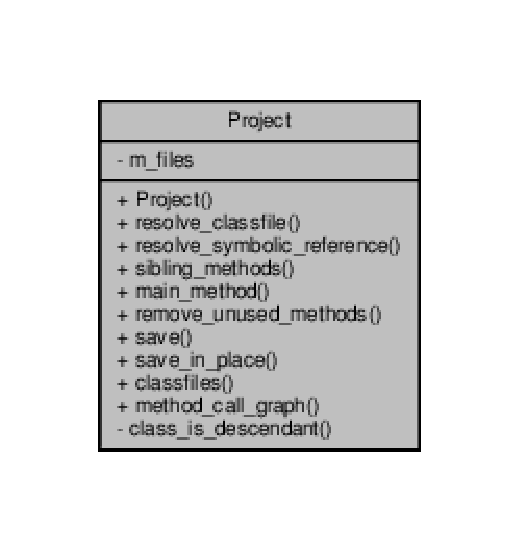
\includegraphics[width=0.5\textwidth]{classProject__coll__graph}
	\caption{Clasa Project}
    \label{fig:classproject}
\end{figure}


Clasa Project se ocupă de operațiile la nivelul întregului proiect - rezolvarea
metodelor simbolice și optimizarea de dimensiune.

Clasa Method corespunde unei singure metode dintr-o clasă.

Metodele care nu sunt descrise în această parte nu au fost considerate suficient
de relevante pentru a fi incluse în teză, iar documentația pentru ele se poate
găsi inline în codul sursă, cât și în documentația generată de Doxygen.

Funcția main\_method~\ref{main_method}, care determină metoda
principală (main entry-point) al proiectului, are antetul
\begin{lstlisting}[language=C++]
Method Project::main_method() const;
\end{lstlisting}

Funcția cand~\ref{cand}, care determină ce funcțiile candidat, este reprezentată de funcția
\begin{lstlisting}[language=C++]
std::vector<Method> Project::sibling_methods(const Method& m) const;
\end{lstlisting}
denumită astfel deoarece am considerat că o metodele
candidat sunt înrudite între ele.

Procedura reachable\_methods\_in\_java~\ref{reachable_methods_in_java} pentru
determinarea funcțiilor accesibile este reprezentată de
\begin{lstlisting}[language=C++]
std::vector<Method> Project::method_call_graph(const Method& m) const;
\end{lstlisting}
denumită astfel pentru a evidenția faptul că mulțimea returnată sunt nodurile
unui graf.

Iar procedura principală
optimize\_for\_size\_in\_java~\ref{optimizeoptimize_for_size_in_java} este
reprezentată de:
\begin{lstlisting}[language=C++]
void Project::remove_unused_methods();
\end{lstlisting}

Procedura from\_symbolic\_reference~\ref{from_symbolic_reference}, folosită
pentru a rezolva referințele simbolice către metode, este reprezentată de
\begin{lstlisting}[language=C++]
static std::optional<Method>
from_symbolic_reference(const ClassFile &file, int cp_index, cp_info info);
\end{lstlisting}

Motivul pentru care această funcție întoarce un \texttt{optional}, în loc de
direct metoda, este că există referințe către funcții terțe, de
obicei definite în librării, care nu pot fi rezolvate în clasele proiectului nostru.
De exemplu, funcția \texttt{println(String s)}, definită în librăria standard
\texttt{java.io}.


